\documentclass[11pt]{article}
\usepackage{fullpage}
\usepackage{url}
\usepackage{stmaryrd}
\usepackage{amssymb}
\usepackage[sans]{dsfont}
\usepackage{color, colortbl}
\usepackage{courier}
\usepackage{graphicx}
\usepackage[all]{xy}
\xyoption{line}

\newcommand{\amr}[1]{\fbox{Amr says:} \textbf{#1}}

% ----------------------------------------------------------------------
% XY-Pic definitions for making ``wire charts''

\def\wirechart#1#2{\let\labelstyle\objectstyle\xy*[*1.0]\xybox{\small%
\xymatrix@C=10mm@R=4mm#1{#2}}\endxy}
\def\wire#1#2{\ar@{-}[#1]^<>(.5){#2}}
\def\wireright#1#2{\wire{#1}{#2}\ar@{}[#1]|<>(.5)/.6ex/{\dir2{>}}}
\def\wireleft#1#2{\wire{#1}{#2}\ar@{}[#1]|<>(.5)/-.6ex/{\dir2{<}}}
\def\wwblank#1{*=<#1,0mm>{~}}
\def\wblank{\wwblank{11mm}}
\def\blank{\wwblank{8mm}}
\def\vublank{*=<0mm,2.3mm>!D{}}
\def\vdblank{*=<0mm,2.3mm>!U{}}
\def\vsblank{*=<0mm,5.6mm>{}}
\def\wirecross#1{\save[]!L;[#1]!R**@{-}\restore}
\def\wirebraid#1#2{\save[]!L;[#1]!R**{}?(#2)**@{-}\restore\save[#1]!R;[]!L**{}?(#2)**@{-}\restore}
\def\wireopen#1{\save[]!R;[#1]!R**\crv{[]!C&[#1]!C}\restore}
\def\wireclose#1{\save[]!L;[#1]!L**\crv{[]!C&[#1]!C}\restore}
\def\wireopenlabel#1#2{\save[]!R;[#1]!R**\crv{[]!C&[#1]!C}?<>(.5)*^+!R{#2}\restore}
\def\wirecloselabel#1#2{\save[]!L;[#1]!L**\crv{[]!C&[#1]!C}?<>(.5)*^+!L{#2}\restore}
\def\wireid{\blank\save[]!L*{};[]!R*{}**@{-}\restore}
\def\wwireid{\wblank\save[]!L*{};[]!R*{}**@{-}\restore}
\def\wwwireid#1{\wwblank{#1}\save[]!L*{};[]!R*{}**@{-}\restore}
\newcommand{\corner}{\rule{2.5mm}{2.5mm}}
\def\minheight{8mm}
\def\addheight{8mm}
\def\cornerbox#1#2#3{  % draw a box with a marked corner around
                   % the object #1. #2=label
                   % usage:   \ulbox{[ll].[].[ul]}{f}
  \save#1="box";
  "box"!C*+<0mm,\addheight>+=<0mm,\minheight>[|(5)]\frm{-}="box1";
  "box1"*{#2};
  ={"box1"!LU*!LU[]{\corner}}"ul";
  ={"box1"!RU*!RU[]{\corner}}"ur";
  ={"box1"!LD*!LD[]{\corner}}"dl";
  ={"box1"!RD*!RD[]{\corner}}"dr";
  #3
  \restore
}
\def\nnbox#1#2{\cornerbox{#1}{#2}{}}
\def\ulbox#1#2{\cornerbox{#1}{#2}{"ul"}}
\def\urbox#1#2{\cornerbox{#1}{#2}{"ur"}}
\def\dlbox#1#2{\cornerbox{#1}{#2}{"dl"}}
\def\drbox#1#2{\cornerbox{#1}{#2}{"dr"}}
\def\ubox#1#2{\cornerbox{#1}{#2}{"ul","ur"}}
\def\dbox#1#2{\cornerbox{#1}{#2}{"dl","dr"}}
\def\lbox#1#2{\cornerbox{#1}{#2}{"ul","dl"}}
\def\rbox#1#2{\cornerbox{#1}{#2}{"ur","dr"}}
\def\circbox#1{*+[o][F-]{#1}}

\newtheorem{definition}{Definition}
\newtheorem{n-lemma}{Lemma}[section]
\newtheorem{n-example}[n-lemma]{Example}
\newenvironment{example}{\begin{n-example}}{\end{n-example}}

\newcommand{\ssep}{\hspace{1em}} 
\newcommand{\sym}{c}       % braid: could be \sigma or c or \gamma
\newcommand{\cp}{\circ}                 % composition
\newcommand{\symi}{\sym\inv}
\newcommand{\inv}{^{-1}}
\newcommand{\id}{\textrm{\rm id}}       % identity
\newcommand{\x}{\otimes}
\newcommand{\boolt}{\mathit{bool}}
\newcommand{\ffv}{\mathit{false}}
\newcommand{\ttv}{\mathit{true}}
\newcommand{\notb}{\mathit{not}}
\newcommand{\union}{\cup}
\newcommand{\transport}[2]{\overline{#1}(#2)}
\newcommand{\refl}{\mathit{refl}}
\renewcommand{\path}{\leadsto}
\newcommand{\paths}[1]{\mathds{P}(#1)}
%% \renewcommand{\circ}{\circlearrowleft}
\newcommand{\alt}{~|~}
\newcommand{\dt}[1]{\llbracket #1 \rrbracket}
\newcommand{\leftv}[1]{\textsf{left}~#1}
\newcommand{\rightv}[1]{\textsf{right}~#1}
\newcommand{\iso}{\leftrightarrow}
\newcommand{\identlp}{\mathit{identl}_+}
\newcommand{\identrp}{\mathit{identr}_+}
\newcommand{\swapp}{\mathit{swap}_+}
\newcommand{\assoclp}{\mathit{assocl}_+}
\newcommand{\assocrp}{\mathit{assocr}_+}
\newcommand{\identlt}{\mathit{identl}_*}
\newcommand{\identrt}{\mathit{identr}_*}
\newcommand{\swapt}{\mathit{swap}_*}
\newcommand{\assoclt}{\mathit{assocl}_*}
\newcommand{\assocrt}{\mathit{assocr}_*}
\newcommand{\distz}{\mathit{dist}_0}
\newcommand{\factorz}{\mathit{factor}_0}
\newcommand{\dist}{\mathit{dist}}
\newcommand{\factor}{\mathit{factor}}
\newcommand{\idc}{\mathit{id}}
\newcommand{\wedgesum}{\vee}
\newcommand{\smashproduct}{\wedge}
\newcommand{\symc}[1]{\mathit{sym}~#1}
\newcommand{\proves}{\vdash}
\newcommand{\Rule}[4]{
\makebox{{\rm #1}
$\displaystyle
\frac{\begin{array}{l}#2\\\end{array}}
{\begin{array}{l}#3\\\end{array}}$
 #4}}
\newcommand{\jdg}[3]{#2 \proves_{#1} #3}

\begin{document}
\begin{titlepage}
\begin{center}
\vfill
{\LARGE Isomorphisms as Groupoids: \\ 
  Homotopy Type Theory and Fractional Types} \\[1.5cm]
{\Large Jacques Carette${}^*$ \qquad Amr Sabry${}^{\dagger}$}\\[0.5cm]
{\Large $({}^*)$~McMaster University \qquad $({}^\dagger)$~Indiana University}
\vfill
\end{center}
\vfill
\noindent\textbf{Abstract.} 

\vfill
\vfill
\end{titlepage}

\title{Isomorphisms as Groupoids: \\ 
  Homotopy Type Theory and Fractional Types}
\author{Jacques Carette \and Amr Sabry}
\date{\today}
\maketitle

%%%%%%%%%%%%%%%%%%%%%%%%%%%%%%%%%%%%%%%%%%%%%%%%%%%%%%%%%%%%%%%%%%%%%%%%%%%%%%
\section{Introduction}

HoTT cannot really deal with functions. The starting point is that paths
explain and witness identities. This works for all the usual types but not
for functions or universes. For functions, the HoTT treatment is to allow
arbitrary functions, single out the isos via classical extensional methods,
and then assert via an axiom that the class of singled out functions is
equivalent to paths. This is a convoluted way. Why not start with functions
that are, by construction, isos. This was the programme we started earlier,
inspired by physical considerations. Because physics requires various
conservation principles (including conservation of information) and because
computation is fundamentally a physical process, the argument (originally due
to Feynman etc.) was that computation should be based on reversible
processes, or in abstract terms, on isomorphisms. That fits very well with
the HoTT philosophy that makes isos first-class. Except that HoTT does not
deal exclusively with isos, the functions are generally not isos. So let's
investigate the radical idea that all functions are isos in the HoTT
framework. What we get is a notion of first-class functions that by
construction are isos and obey the usual path rules etc. The technical device
is the notion of fractional types which are dual to products. A function
(iso) $A \rightarrow B$ is represented as an element of the type
$(\frac{1}{A} \times B)$. The construction shows the essential nature of the
$\infty$-groupoid structure. The more higher-order functions we have the
higher we have to go in the groupoid structure. We also have something
significant in the realm of reversible computing. We finally have
higher-order functions. Of course we need to show that we have constructed a
monoidal closed category (a concrete one) and then we can inherit all the
fancy constructions. Finally we have a very interesting operational
interpretation of paths and we outline various applications.

Need a clear explanation of why we can't deal with the usual functions that
are not isomorphisms. Regular function spaces obey $1^A = 1$ for all $A$. In
terms of fractionals this gives $\frac{1}{A} = 1$ for all $A$ which is not
true. However if we restrict to isomorphisms then the only functions we can
write are $A \rightarrow B$ where $A$ and $B$ are isomorphic types and hence
the only functions we can write in the space $1^A$ are to types $A$ that are
isomorphic to 1 and in that case we do indeed get that $\frac{1}{A} =
1$. See~\cite{fiore-remarks} for more details. The benefit is that we fit
squarely in the physically motivated notion that isomorphisms are the
foundational computational mechanism as well as the HoTT approach that is
essentially all about isomorphisms. Of course we don't lose anything by
restricting our attention to isomorphisms because we know that general
(irreversible) functions can be obtained from isomorphisms via
\emph{information effects}~\cite{James:2012:IE:2103656.2103667}.

We are witnessing a convergence of ideas from several distinct research
communities (physics, mathematics, and computer science) towards replacing
\emph{equalities} by \emph{isomorphisms}. The combined programme has sparked
a significant amount of research that unveiled new and surprising connections
between geometry, algebra, logic, and computation (see~\cite{baez2011physics}
for an overview of some of the connections).

In the physics community, Landauer~\cite{Landauer:1961,Landauer},
Feynman~\cite{springerlink:10.1007/BF02650179}, and others have interpreted
the laws of physics as fundamentally related to computation. The great
majority of these laws are formulated as equalities between different
physical observables which is unsatisfying: \emph{different} physical
observables should not be related by an \emph{equality}. It is more
appropriate to relate them by an \emph{isomorphism} that witnesses, explains,
and models the process of transforming one observable to the other.

In the mathematics and logic community, Martin-L\"of developed an extension
of the simply typed $\lambda$-calculus originally intended to provide a
rigorous framework for constructive
mathematics~\cite{citeulike:7374951}. This theory has been further extended
with \emph{identity types} representing the proposition that two terms are
``equal.'' (See~\cite{streicher,warren} for a survey.) Briefly speaking,
given two terms $a$ and $b$ of the same type $A$, one forms the type
$\texttt{Id}_A(a,b)$ representing the proposition that~$a$ and~$b$ are equal:
in other words, a term of type $\texttt{Id}_A(a,b)$ witnesses, explains, and
models the process of transforming $a$ to $b$ and vice-versa.

In the computer science community, the theory and practice of type
isomorphisms is well-established. Originally, such type isomorphisms were
motivated by the pragmatic concern of searching large libraries of functions
by providing one of the many possible isomorphic types for the desired
function~\cite{Rittri:1989:UTS:99370.99384}. More recently, type isomorphisms
have taken a more central role as \emph{the} fundamental computational
mechanism from which more conventional, i.e., irreversible computation, is
derived. In our own previous
work~\cite{James:2012:IE:2103656.2103667,rc2011,rc2012} we started with the
notion of type isomorphism and developed from it a family of programming
languages, $\Pi$ with various superscripts, in which computation is an
isomorphism preserving the information-theoretic entropy.

A major open problem remains, however: a higher-order extension of
$\Pi$. This extension is of fundamental importance in all the originating
research areas. In physics, it allows for quantum states to be viewed as
processes and processes to be viewed as states, such as with the
Choi-Jamiolkowski
isomorphism~\cite{choi1975completely,jamiolkowski1972linear}.  In mathematics
and logic, it allows the equivalence between different proofs of type
$\texttt{Id}_A(a,b)$ to itself be expressed as an isomorphism (of a higher
type) $\texttt{Id}_{\texttt{Id}_A(a,b)}(p,q)$. Finally, in computer science,
higher-order types allow code to abstract over other code fragments as well
as the manipulation of code as data and data as code.

Technically speaking, obtaining a higher-order extension requires the
construction of a \emph{closed category} from the underlying monoidal
category for~$\Pi$. Although the general idea of such a construction is
well-understood, the details of adapting it to an actual programming language
are subtle.  Our main novel technical device to achieving the higher-order
extension is a \emph{fractional type} which represents \emph{negative
information} and which is so named because of its duality with conventional
product types.

From the wikipedia page on homeomorphism: 
\begin{quote}
The intuitive criterion of stretching, bending, cutting and gluing back
together takes a certain amount of practice to apply correctly—it may not be
obvious from the description above that deforming a line segment to a point
is impermissible, for instance. It is thus important to realize that it is
the formal definition given above that counts.

This characterization of a homeomorphism often leads to confusion with the
concept of homotopy, which is actually defined as a continuous deformation,
but from one function to another, rather than one space to another. In the
case of a homeomorphism, envisioning a continuous deformation is a mental
tool for keeping track of which points on space X correspond to which points
on Y—one just follows them as X deforms. In the case of homotopy, the
continuous deformation from one map to the other is of the essence, and it is
also less restrictive, since none of the maps involved need to be one-to-one
or onto. Homotopy does lead to a relation on spaces: homotopy equivalence.

There is a name for the kind of deformation involved in visualizing a
homeomorphism. It is (except when cutting and regluing are required) an
isotopy between the identity map on X and the homeomorphism from X to Y.
\end{quote}

It is strange for homotopy type theory to be all about isomorphisms and then
not insist on isomorphisms between spaces.

If we focus on homeomorphisms, the higher-order space is a \emph{torsor}.

%%%%%%%%%%%%%%%%%%%%%%%%%%%%%%%%%%%%%%%%%%%%%%%%%%%%%%%%%%%%%%%%%%%%%%%%%%%%%%
\section{Intuitive Ideas and Examples} 
\label{sec:intuition}

%% the next 7 figures are taken from Selinger's paper on graphical languages
%% for monoidal categories; if we use them make sure it's ok with him and
%% acknowledge him

In homotopy type theory, there is a focus on isomomorphisms represented by
paths (proofs of identities) and yet arbitrary functions are considered. We
propose to only consider functions that are themselves isomorphisms: this
will allow us to view the function itself as a collection of paths and it
doesn't lose anything in terms of computability because we know that we could
do everything with reversible functions if we wanted to.

Consider the function $\notb$ from the space $\boolt$ to itself. We can
represent this function as a pair of paths. Since we are in a topological
world, we should care whether the path top pass crosses over the bottom one
or vice-versa. In the diagram below, we chose for the top wire to cross over
the bottom one:

\begin{center}
  \begin{tabular}{@{}llc@{}}
    $\notb : \boolt \rightarrow \boolt$ & & 
    $\vcenter{\wirechart{@C=1.5cm@R=0.8cm}{
        *{}\wireright{r}{\ffv}&\blank\wirecross{d}\wireright{r}{\ffv}&\\
        *{}\wireright{r}{\ttv}&\blank\wirebraid{u}{.3}\wireright{r}{\ttv}&
        }}$ 
  \end{tabular}
\end{center}

It is important also to note that the two paths must be taken together
because there is a constraint between them. If the top path takes $\ffv$ to
$\ttv$ then the bottom path cannot take $\ttv$ to $\ttv$: it \emph{has} to
lead to $\ffv$. We will return to this point later.

For now, consider the functions:
\[\begin{array}{rcl}
\mathit{id}^1 &=& \lambda x.x \\
\mathit{id}^2 &=& \lambda x. \notb~(\notb~x)
\end{array}\]
These two functions are evidently extensionally equivalent and hence in the
conventional treatment of homotopy type theory, it is acceptable to assume
they are also propositionally equivalent, i.e., it is acceptable to postulate
a path $\mathit{id}^1 \path \mathit{id}^2$ in the space $\boolt \rightarrow
\boolt$. 

When represented as paths, we get the following situation for the second
function:
\[\vcenter{\wirechart{@C=1.5cm@R=0.8cm}{
    *{}\wireright{r}{\ffv}&
    \blank\wirecross{d}\wireright{r}{\ffv}&
    \blank\wirecross{d}\wireright{r}{\ffv}&
    \\
    *{}\wireright{r}{\ttv}&
    \blank\wirebraid{u}{.3}\wireright{r}{\ttv}&
    \blank\wirebraid{u}{.3}\wireright{r}{\ttv}&
    \\
    }}
\]
Repeating the $\notb$ operation results in a twisted path that externally
behaves like the identity but that evidently not identical to the straight
path with no twists. Thus although one can justify that the two functions
should have a path between them, the function extensionality axiom does not
give insights into \emph{what} this path is actually doing topologically.















%% \begin{center}
%%   \begin{tabular}{@{}llc@{}}
%%     Braiding & $\sym_{A,B}$ &
%%     $\vcenter{\wirechart{@C=1.5cm@R=0.8cm}{
%%         *{}\wireright{r}{B}&\blank\wirecross{d}\wireright{r}{A}&\\
%%         *{}\wireright{r}{A}&\blank\wirebraid{u}{.3}\wireright{r}{B}&
%%         }}$ \\
%%   \end{tabular}
%% \end{center}

%% Note that the braiding satisfies
%% $\sym_{A,B}\cp\symi_{A,B}=\id_{A\x B}$, but not
%% $\sym_{A,B}\cp\sym_{B,A}=\id_{A\x B}$. Graphically:

%% \[\vcenter{\wirechart{@C=1.5cm@R=0.8cm}{
%%     *{}\wireright{r}{B}&
%%     \blank\wirecross{d}\wireright{r}{A}&
%%     \blank\wirebraid{d}{.3}\wireright{r}{B}&
%%     \\
%%     *{}\wireright{r}{A}&
%%     \blank\wirebraid{u}{.3}\wireright{r}{B}&
%%     \blank\wirecross{u}\wireright{r}{A}&
%%     \\
%%     }}
%% = \id_{A\x B},
%% \]
%% \[\vcenter{\wirechart{@C=1.5cm@R=0.8cm}{
%%     *{}\wireright{r}{B}&
%%     \blank\wirecross{d}\wireright{r}{A}&
%%     \blank\wirecross{d}\wireright{r}{B}&
%%     \\
%%     *{}\wireright{r}{A}&
%%     \blank\wirebraid{u}{.3}\wireright{r}{B}&
%%     \blank\wirebraid{u}{.3}\wireright{r}{A}&
%%     \\
%%     }}
%% \neq \id_{A\x B}.
%% \]

%% \begin{example}
%%   The hexagon axiom translates into the following in the graphical
%%   language:

%%   \[ (\id_B\x\sym_{A,C}) \cp \alpha_{B,A,C} \cp (\sym_{A,B}\x\id_C)
%%   = \alpha_{B,C,A} \cp (\sym_{B,C\x A}) \cp \alpha_{A,B,C}
%%   \]
%%   \[\vcenter{\wirechart{@R=6mm}{
%%     \wireright{r}{C}&
%%     \wireid\wireright{r}{C}&
%%     \blank\wirecross{d}{.3}\wireright{r}{A}&
%%     \\
%%     \wireright{r}{B}&
%%     \blank\wirecross{d}{.3}\wireright{r}{A}&
%%     \blank\wirebraid{u}{.3}\wireright{r}{C}&
%%     \\
%%     \wireright{r}{A}&
%%     \blank\wirebraid{u}{.3}\wireright{r}{B}&
%%     \wireid\wireright{r}{B}&
%%     \\
%%     }}
%%   \ssep=\ssep
%%   \vcenter{\wirechart{@R=6mm}{
%%     \wireright{r}{C}&
%%     \blank\wirecross{d}{.3}\wireright{r}{A}&
%%     \\
%%     \wireright{r}{B}&
%%     \blank\wirecross{d}{.3}\wireright{r}{C}&
%%     \\
%%     \wireright{r}{A}&
%%     \blank\wirebraid{uu}{.2}\wireright{r}{B}&
%%     \\
%%     }}
%%   \]
%% \end{example}

%% \begin{example}
%%   The {\em Yang-Baxter equation} is the following equation, which is a
%%   consequence of the hexagon axiom and naturality:
%%   \[ (\sym_{B,C}\x\id_A)\cp(\id_B\x\sym_{A,C})\cp(\sym_{A,B}\x\id_C) =
%%   (\id_C\x\sym_{A,B})\cp(\sym_{A,C}\x\id_B)\cp(\id_A\x\sym_{B,C}).
%%   \]
%%   In the graphical language, it becomes:
%%   \[\vcenter{\wirechart{@C-4mm@R=6mm}{
%%     \wireright{r}{C}&
%%     \wireid\wireright{r}{C}&
%%     \blank\wirecross{d}{.3}\wireright{r}{A}&
%%     \wireid\wireright{r}{A}&
%%     \\
%%     \wireright{r}{B}&
%%     \blank\wirecross{d}{.3}\wireright{r}{A}&
%%     \blank\wirebraid{u}{.3}\wireright{r}{C}&
%%     \blank\wirecross{d}{.3}\wireright{r}{B}&
%%     \\
%%     \wireright{r}{A}&
%%     \blank\wirebraid{u}{.3}\wireright{r}{B}&
%%     \wireid\wireright{r}{B}&
%%     \blank\wirebraid{u}{.3}\wireright{r}{C}&
%%     \\
%%     }}
%%   \ssep=\ssep
%%   \vcenter{\wirechart{@C-4mm@R=6mm}{
%%     \wireright{r}{C}&
%%     \blank\wirecross{d}{.3}\wireright{r}{B}&
%%     \wireid\wireright{r}{B}&
%%     \blank\wirecross{d}{.3}\wireright{r}{A}&
%%     \\
%%     \wireright{r}{B}&
%%     \blank\wirebraid{u}{.3}\wireright{r}{C}&
%%     \blank\wirecross{d}{.3}\wireright{r}{A}&
%%     \blank\wirebraid{u}{.3}\wireright{r}{B}&
%%     \\
%%     \wireright{r}{A}&
%%     \wireid\wireright{r}{A}&
%%     \blank\wirebraid{u}{.3}\wireright{r}{C}&
%%     \wireid\wireright{r}{C}&
%%     \\
%%     }}
%%   \]
%% \end{example}

Talk about groupoid cardinality and give an example of how the cardinality of
a group of order $n$ is $\frac{1}{n}$.

%%%%%%%%%%%%%%%%%%%%%%%%%%%%%%%%%%%%%%%%%%%%%%%%%%%%%%%%%%%%%%%%%%%%%%%%%%%%%%
\section{The Category of Pointed Groupoids}

%%%%%%%%%%%%%%%%%
\subsection{Paths} 

\begin{definition}[Path]
A \emph{path} $p : x \path y$ between two points $x$ and $y$ in some space
$A$ is a directed edge $p$ from $x$ to $y$. We denote the set of paths of the
space $A$ as $\paths{A}$.
\end{definition}

\begin{definition}[Disjoint union of paths]
Given $\paths{A}$ and $\paths{B}$ in spaces $A$ and $B$ respectively, we
construct $\paths{A} \uplus^p \paths{B}$ in space $A \uplus B$, the disjoint
union of $A$ and $B$, as follows:
\[ 
  \{ \leftv{p} : \leftv{x} \path \leftv{y} ~|~ 
    (p : x \path y) \in \paths{A} \}
  \union
  \{ \rightv{q} : \rightv{x} \path \rightv{y} ~|~ 
    (q : x \path y) \in \paths{B} \}
\]
\end{definition}
We will sometimes write this as $\leftv{(\paths{A})} \union
\rightv{(\paths{B})}$.

\begin{definition}[Product of paths]
Given $\paths{A}$ and $\paths{B}$ in spaces $A$ and $B$
respectively, we construct $\paths{A} \times^p \paths{B}$ in
space $A \times B$, the cartesian product of $A$ and $B$, as follows: 
\[ 
\{ (p,q) : (x,z) \path (y,w) ~|~ (p : x \path y) \in \paths{A}, 
   (q : z \path w) \in \paths{B} \}
\]
\end{definition}
We will sometimes write this as $(\paths{A},\paths{B})$.

%%%%%%%%%%%%%%%%%
\subsection{Pointed Groupoids} 

\begin{definition}[Groupoid]
A \emph{groupoid} $G = (G_0, \paths{G_0})$ is a set $G_0$ together
with a collection of paths $x \path y$, between elements $x$ and $y$ of $G_0$
that satisfies the following conditions:
\begin{itemize}
\item for every $x \in G_0$, there is a path $\refl_x : x \path x$,
\item every path $p : x \path y$, there is an inverse path $! p : y \path x$, 
\item for every paths $p : x \path y$ and $q : y \path z$ there is a path $p
  \circ q : x \path z$, and
\item for every paths $p : x \path y$, $q : y \path z$, and $r : z \path w$,
  we have:
  \begin{itemize}
  \item $\refl_x \circ p = p$;
  \item $p \circ \refl_y = p$;
  \item $(p \circ q) \circ r = (p \circ (q \circ r))$;
  \item $p \,\circ\, !p = \refl_x$;
  \item $!p \,\circ\, p = \refl_y$.
  \end{itemize}
\end{itemize}
\end{definition}
When introducing a groupoid, we only explicitly mention a collection of
non-trivial ``generating'' paths. The equivalence closure under $\refl$, $!$,
and $\circ$ with the appropriate conditions is implicitly
assumed.\footnote{For higher groupoids, the five equivalences in the last
  condition will be witnessed by paths between paths and not by the
  extensional equivalence relation $=$.}

\begin{definition}[Pointed groupoid]
A pointed groupoid $G_{\bullet} = (G_0, \bot_{G_0}, \paths{G_0})$ is
a groupoid $(G_0, \paths{G_0})$ with a distinguished element
$\bot_{G_0} \in G_0$.
\end{definition}

\begin{definition}[Wedge sum]
The \emph{wedge sum} of two pointed groupoids $G_\bullet$ and $H_\bullet$,
written $G_\bullet \wedgesum H_\bullet$ is defined as follows:
\[\begin{array}{l}
(G_0, \bot_{G_0}, \paths{G_0}) \wedgesum 
(H_0, \bot_{H_0}, \paths{H_0}) = \\
((G_0 \uplus H_0) \union \{ \bot \},
 \bot,
 (\paths{G_0} \uplus^p \paths{H_0}) \union
 \{ L: \leftv{\bot_{G_0}} \path \bot, 
    R: \rightv{\bot_{H_0}} \path \bot \})
\end{array}\]
where $\uplus$ is the disjoint union operation on sets and $\bot$ is a new
distinguished element that is related by new paths to the distinguished
elements of $G_\bullet$ and $H_\bullet$.
\end{definition}

\begin{definition}[Smash product]
The \emph{smash product} of two pointed groupoids $G_\bullet$ and
$H_\bullet$, written $G_\bullet \smashproduct H_\bullet$ is defined as
follows:
\[\begin{array}{l}
(G_0, \bot_{G_0}, \paths{G_0}) \smashproduct
(H_0, \bot_{H_0}, \paths{H_0}) = \\
((G_0 \times H_0) \union \{ \bot \},
 \bot,
 (\paths{G_0} \times^p \paths{H_0}) \union
 \{ F_h: (\bot_{G_0},h) \path \bot \} \union 
 \{ S_g: (g,\bot_{H_0}) \path \bot \} 
\end{array}\]
where $\times$ is the cartesian product operation on sets and $\bot$ is a new
distinguished element that is related by new paths to every pair of elements
that includes either $\bot_{G_0}$ or $\bot_{H_0}$. 
\end{definition}

\begin{definition}[Denotation of types]
Each type $b$ is mapped to a \emph{pointed groupoid} $(\dt{b}, \bot_b,
\paths{b})$ as follows:
\[\begin{array}{rcl@{\qquad}l}
\dt{0} &=& (\{ \bot_0 \}, \bot_0, \{ \mathit{loop}_0 : \bot_0 \path \bot_0 \}) &
           (\mbox{circle}) \\
\dt{1} &=& (\{ \bullet, \bot_1 \}, \bot_1, 
           \{ \mathit{loop}_1 : \bot_1 \path \bot_1 \}) &\\
\dt{(b_1 + b_2)} &=& \dt{b_1} \wedgesum \dt{b_2} & 
           (\mbox{wedge~sum}) \\
\dt{(b_1 * b_2)} &=& \dt{b_1} \smashproduct \dt{b_2} & 
           (\mbox{smash~product})
\end{array}\]
\end{definition} 

Topologically $\dt{0}$ corresponds to the circle $S^1$ which has Euler
characteristic (which generalizes the notion of set cardinality) of 0. As a
groupoid, the space $\dt{0}$ includes this infinite collection of paths from
$\bot_0 \path \bot_0$:
\[\begin{array}{l}
\refl_{\bot_0} \\
\mathit{loop}_0 \\
!~\mathit{loop}_0 \\
\mathit{loop}_0 \circ \mathit{loop}_0 \\
!~(\mathit{loop}_0 \circ \mathit{loop}_0) \\
\mathit{loop}_0 \circ \mathit{loop}_0 \circ \mathit{loop}_0 \\
!~(\mathit{loop}_0 \circ \mathit{loop}_0 \circ \mathit{loop}_0) \\
\vdots
\end{array}\]
and hence, using the definition introduced by Baez and
Dolan~\cite{groupoidcard}, has groupoid cardinality 0. We will abbreviate
this collection of paths as $\mathit{loop}^n_0$ for integer $n$, where
$\mathit{loop}^0_0$ is $\refl$, and $\mathit{loop}^n_0$ abbreviates the
$n$-fold composition in one direction for positive $n$ and in the opposite
direction for negative $n$.

Note that all our pointed spaces have a similar structure: a collection of
``regular elements'' forming several connected components and a separate
isolated connected component that includes the distinguished element
$\bot$. The distinguished element $\bot$ has the infinite collection of loops
on it and, in general, may be connected to the distinguished elements of the
subspaces used in the construction. That entire cluster including $\bot$ has
Euler characteristic and groupoid cardinality 0.

We now check that the wedge sum of any of our pointed groupoids $G_\bullet$
with $\dt{0}$ is ``essentially'' $G_\bullet$ itself, i.e., that $\dt{0}$ is
the additive unit in our space of pointed groupoids. Consider:
\[\begin{array}{l}
G_\bullet \wedgesum \dt{0} = \\
(G_0, \bot_{G_0}, \paths{G_0}) \wedgesum 
  (\{ \bot_0 \}, \bot_0, \{ \mathit{loop}_0 : \bot_0 \path \bot_0 \}) = \\
((\leftv{G_0} \union \{ \rightv{\bot_0}, \bot \}, 
 \bot,
 (\leftv{\paths{G_0}} \union \{ \rightv{\mathit{loop}^n_0} , 
 \leftv{\bot_{G_0}} \path \bot, \rightv{\bot_0} \path \bot \})
\end{array}\]
One can see that this space consists of $\leftv{G_0}$ with whatever structure
is on it and another connected component consisting of $\leftv{\bot_{G_0}}$,
$\rightv{\bot_0}$, and the new $\bot$ for the entire space. This cluster has
cardinality 0 and hence the new space is ``equivalent'' to the original
$G\bullet$ as we have essentially only changed the representation of 0. 

Therefore, since the wedge sum is evidently commutative and associative, it
is at least plausible that the structure $(\wedgesum, \dt{0}$ is a symmetric
monoidal category. All of that will be formalized later. The categorical
morphisms must obviously map distinguished elements to distinguished elements
and preserve the structure of the path. It is also reasonably easy to see
that the structure $(\smashproduct, \dt{1})$ is another symmetric monoidal
category. Even better one can check that for any pointed groupoid
$G_\bullet$, we have $G_\bullet \smashproduct \dt{0}$ gives us a very
complicated 0 but still a 0. I didn't check distributivity but I suspect it
holds too.

%%%%%%%%%%%%%%%%%%%%%%%%%%%%%%%%%%%%%%%%%%%%%%%%%%%%%%%%%%%%%%%%%%%%%%%%%%%%%%
\section{Finite Types as Pointed Groupoids} 

We review our language $\Pi$ providing the necessary background and context
for our higher-order extension.\footnote{The presentation in this section
  focuses on the simplest version of $\Pi$. Other versions include recursive
  types and trace operators but these extensions are orthogonal to the
  higher-order extension emphasized in this document.} Even though the
semantics of $\Pi$ could be explained using plain sets, we express it using
the groupoid terminology to facilitate the transition to fractionals and
higher-order functions. 

%%%%%%%%%%%%%%%%%
\subsection{Syntax and Types} 

The terms of $\Pi$ are not classical values and functions; rather, the terms
are isomorphism witnesses.  In other words, the terms of $\Pi$ are proofs
that certain ``shapes of values'' are isomorphic.  And, in classical
Curry-Howard fashion, our operational semantics shows how these proofs can be
directly interpreted as actions on ordinary values which effect this shape
transformation. Of course, ``shapes of values'' are very familiar already:
they are usually called \emph{types}.  But frequently one designs a type
system as a method of classifying terms, with the eventual purpose to show
that certain properties of well-typed terms hold, such as safety.  Our
approach is different: we start from a type system, and then present a term
language which naturally inhabits these types, along with an appropriate
operational and denotational semantics.

\paragraph*{Data.}
We view $\Pi$ as having two levels: it has traditional values classified by
ordinary types:
\[\begin{array}{rcl} 
\textit{values}, v &::=& () \alt \leftv{v} \alt \rightv{v} \alt (v,v) \\
\textit{value types}, b &::=& 0 \alt 1 \alt b+b \alt b * b
\end{array}\]

Types include the empty type $0$, the unit type $1$, sum types $b_1+b_2$, and
product types $b_1*b_2$.  Values include $()$ which is the only value of type
$1$, $\leftv{v}$ and $\rightv{v}$ which inject $v$ into a sum type, and
$(v_1,v_2)$ which builds a value of product type.

\paragraph*{Isomorphisms.} The terms of $\Pi$ witness
type isomorphisms of the form $b \iso b$. They consist of base isomorphisms,
as defined below, and their composition.
\[\begin{array}{rrcll}
\identlp :&  0 + b & \iso & b &: \identrp \\
\swapp :&  b_1 + b_2 & \iso & b_2 + b_1 &: \swapp \\
\assoclp :&  b_1 + (b_2 + b_3) & \iso & (b_1 + b_2) + b_3 &: \assocrp \\
\identlt :&  1 * b & \iso & b &: \identrt \\
\swapt :&  b_1 * b_2 & \iso & b_2 * b_1 &: \swapt \\
\assoclt :&  b_1 * (b_2 * b_3) & \iso & (b_1 * b_2) * b_3 &: \assocrt \\
\distz :&~ 0 * b & \iso & 0 &: \factorz \\
\dist :&~ (b_1 + b_2) * b_3 & \iso & (b_1 * b_3) + (b_2 * b_3)~ &: \factor
\end{array}\]

Each line of the above table introduces a pair of dual
constants\footnote{where $\swapp$ and $\swapt$ are self-dual.} that witness
the type isomorphism in the middle.  These are the base (non-reducible) terms
of the second, principal level of $\Pi$. Note how the above has two readings:
first as a set of typing relations for a set of constants. Second, if these
axioms are seen as universally quantified, orientable statements, they also
induce transformations of the (traditional) values. The (categorical or
homotopical) intuition here is that these axioms have computational content
because they witness isomorphisms rather than merely stating an extensional
equality.

The isomorphisms are extended to form a congruence relation by adding the
following constructors that witness equivalence and compatible closure:

\begin{table}[t]
\hrule\medskip
\begin{center} 
\Rule{}
{}
{\jdg{}{}{\idc : b \iso b}}
{}
\quad 
\Rule{}
{\jdg{}{}{c : b_1 \iso b_2}}
{\jdg{}{}{\symc{c} : b_2 \iso b_1}}
{}
\quad
\Rule{}
{\jdg{}{}{c_1 : b_1 \iso b_2} \quad c_2 : b_2 \iso b_3}
{\jdg{}{}{c_1 \fatsemi c_2 : b_1 \iso b_3}}
{}
\\ \bigskip
\Rule{}
{\jdg{}{}{c_1 : b_1 \iso b_2} \quad c_2 : b_3 \iso b_4}
{\jdg{}{}{c_1 \oplus c_2 : b_1 + b_3 \iso b_2 + b_4}}
{}
\quad 
\Rule{}
{\jdg{}{}{c_1 : b_1 \iso b_2} \quad c_2 : b_3 \iso b_4}
{\jdg{}{}{c_1 \otimes c_2 : b_1 * b_3 \iso b_2 * b_4}}
{}
\end{center}
\caption{Combinators\label{pi-combinators}}
\medskip\hrule
\end{table}

It is important to note that ``values'' and ``isomorphisms'' are completely
separate syntactic categories which do not intermix. The semantics of the
language come when these are made to interact at the ``top level'' via
\emph{application}: 
\[\begin{array}{lrcl}
\textit{top level term}, l &::=& c~v
\end{array}\]

%%%%%%%%%%%%%%%%%
\subsection{Groupoid Semantics}

The language presented above, at the type level, models a \emph{commutative
  semiring} (occasionally called a \emph{commutative rig}) where we replace
equality by isomorphism.  Semantically, $\Pi$ models a \emph{bimonoidal
  category} whose simplest example is the category of finite sets and
bijections. In that interpretation, each value type denotes a finite set of a
size calculated by viewing the types as natural numbers and each combinator
$c : b_1 \iso b_2$ denotes a bijection between the sets denoted by $b_1$ and
$b_2$. Instead of presenting such a semantics, we present a more involved
semantics using groupoids. 

The semantics of $\Pi$ is given using two mutually recursive interpreters:
one going forward and one going backwards. The use of $\symc{}$ switches
control from one evaluator to the other.

\[\begin{array}{rcl}
\mathit{eval} &:& (a \iso b) \rightarrow \dt{a} \rightarrow \dt{b} \\
\mathit{eval}~\idc~a &=& a \\
\mathit{eval}~(\symc{f})~b &=& \mathit{evalR}~f~b \\
\mathit{eval}~(f \fatsemi g)~a &=& \mathit{eval}~g~(\mathit{eval}~f~a) \\
\mathit{eval}~(f \otimes g)~(a,b) &=& (\mathit{eval}~f~a, \mathit{eval}~g~b) \\
\mathit{eval}~(f \oplus g)~(\leftv{a}) &=& \leftv{(\mathit{eval}~f~a)} \\
\mathit{eval}~(f \oplus g)~(\rightv{b}) &=& \rightv{(\mathit{eval}~g~b)} \\
\mathit{eval}~\identlp~(\leftv{\circ}) &=& \circ \\
\mathit{eval}~\identlp~(\rightv{a}) &=& a \\
\mathit{eval}~\identrp~a &=& \rightv{a} \\
\mathit{eval}~\swapp~(\leftv{a}) &=& \rightv{a} \\
\mathit{eval}~\swapp~(\rightv{b}) &=& \leftv{b} \\
\mathit{eval}~\assoclp~(\leftv{a}) &=& \leftv{(\leftv{a})} \\
\mathit{eval}~\assoclp~(\rightv{(\leftv{b})}) &=& \leftv{(\rightv{b})} \\
\mathit{eval}~\assoclp~(\rightv{(\rightv{c})}) &=& \rightv{c} \\
\mathit{eval}~\assocrp~(\leftv{(\leftv{a})}) &=& \leftv{a} \\
\mathit{eval}~\assocrp~(\leftv{(\rightv{b})}) &=& \rightv{(\leftv{b})} \\
\mathit{eval}~\assocrp~(\rightv{c}) &=& \rightv{(\rightv{c})} \\
\mathit{eval}~\identlt~((), a) &=& a \\
\mathit{eval}~\identrt~a &=& ((), a) \\
\mathit{eval}~\swapt~(a,b) &=& (b,a) \\
\mathit{eval}~\assoclt~(a,(b,c)) &=& ((a,b),c) \\
\mathit{eval}~\assocrt~((a,b),c)  &=& (a,(b,c)) \\
\mathit{eval}~\distz~(\rightv{c}, a) &=& \rightv{(c, a)} \\
\mathit{eval}~\factorz~(\leftv{(b, a)}) &=& (\leftv{b}, a) \\
\mathit{eval}~\dist~(\leftv{b}, a) &=& \leftv{(b, a)} \\
\mathit{eval}~\dist~(\rightv{c}, a) &=& \rightv{(c, a)} \\
\mathit{eval}~\factor~(\leftv{(b, a)}) &=& (\leftv{b}, a) \\
\mathit{eval}~\factor~(\rightv{(c, a)}) &=& (\rightv{c}, a) \\
\end{array}\]
\[\begin{array}{rcl}
\mathit{evalR} &:& (a \iso ) \rightarrow b \rightarrow a \\
\mathit{evalR}~\idc~a &=& a \\
\mathit{evalR}~(\symc{f}) b &=& \mathit{eval}~f b \\
\mathit{evalR}~(f \fatsemi g) a &=& \mathit{evalR}~f (\mathit{evalR}~g a) \\
\mathit{evalR}~(f \otimes g) (a,b) &=& 
  (\mathit{evalR}~f a, \mathit{evalR}~g b) \\
\mathit{evalR}~(f \oplus g) (\leftv{a}) &=& \leftv{(\mathit{evalR}~f a)} \\
\mathit{evalR}~(f \oplus g) (\rightv{b}) &=& \rightv{(\mathit{evalR}~g b)} \\
\mathit{evalR}~\identlp~a &=& \rightv{a} \\
\mathit{evalR}~\identrp~(\rightv{a}) &=& a \\
\mathit{evalR}~\swapp~(\leftv{a}) &=& \rightv{a} \\
\mathit{evalR}~\swapp~(\rightv{b}) &=& \leftv{b} \\ 
\mathit{evalR}~\assoclp~(\leftv{(\leftv{a})}) &=& \leftv{a} \\
\mathit{evalR}~\assoclp~(\leftv{(\rightv{b})}) &=& \rightv{(\leftv{b})} \\
\mathit{evalR}~\assoclp~(\rightv{c}) &=& \rightv{(\rightv{c})} \\
\mathit{evalR}~\assocrp~(\leftv{a}) &=& \leftv{(\leftv{a})} \\
\mathit{evalR}~\assocrp~(\rightv{(\leftv{b})}) &=& \leftv{(\rightv{b})} \\
\mathit{evalR}~\assocrp~(\rightv{(\rightv{c})}) &=& \rightv{c} \\
\mathit{evalR}~\identlt~a &=& ((), a) \\
\mathit{evalR}~\identrt~((), a) &=& a \\
\mathit{evalR}~\swapt~(a,b) &=& (b,a) \\
\mathit{evalR}~\assoclt~((a,b),c)  &=& (a,(b,c)) \\
\mathit{evalR}~\assocrt~(a,(b,c)) &=& ((a,b),c) \\
\mathit{eval}~\distz~(\rightv{c}, a) &=& \rightv{(c, a)} \\
\mathit{eval}~\factorz~(\leftv{(b, a)}) &=& (\leftv{b}, a) \\
\mathit{evalR}~\dist~(\leftv{(b, a)}) &=& (\leftv{b}, a) \\
\mathit{evalR}~\dist~(\rightv{(c, a)}) &=& (\rightv{c}, a) \\
\mathit{evalR}~\factor~(\leftv{b}, a) &=& \leftv{(b, a)} \\
\mathit{evalR}~\factor~(\rightv{c}, a) &=& \rightv{(c, a)}
\end{array}\]

We state without proof that the evaluation of well-typed combinators always
terminates and that $\Pi$ is logically reversible, i.e., that for all
combinators $c : b_1 \iso b_2$ and values $v_1 : b_1$ and $v_2 : b_2$ we have
the forward evaluation of $c v_1$ produces $v_2$ iff the backwards evaluation
of $c v_2$ produces $v_1$.

%%%%%%%%%%%%%%%%%%%%%%%%%%%%%%%%%%%%%%%%%%%%%%%%%%%%%%%%%%%%%%%%%%%%%%%%%%%%%%
\section{Fractional Types as Groupoids} 

In the previous section, every type was modeled by a collection of values
(including a special ``unusable'' value $\bot$) and a collection of trivial
paths. In this section, non-trivial paths will emerge to model ``fractional
values.'' The intuition is that two values that are connected by a path
should not be counted twice as the path induces an equivalence between these
two values: ``they are the same.'' As illustrated in
Sec.~\ref{sec:intuition}, this idea generalizes to conclude that a value
connected to itself using several paths corresponds to a ``fraction.''

We begin by investigating the special situation of a type $\frac{1}{A}$ where
$A$ is a 0-type (i.e., where $A$ does not contain any fractional components).

%%%%%%%%%%%%%%%%%%%%%%%%%%%%%%%%%%%%%%%%%%%%%%%%%%%%%%%%%%%%%%%%%%%%%%%%%%%%%%
\section{Rank-1 Isomorphisms as 1-Groupoids}

%%%%%%%%%%%%%%%%%%%%%%%%%%%%%%%%%%%%%%%%%%%%%%%%%%%%%%%%%%%%%%%%%%%%%%%%%%%%%%
\section{Rank-$n$ Isomorphisms as $n$-Groupoids}

%%%%%%%%%%%%%%%%%%%%%%%%%%%%%%%%%%%%%%%%%%%%%%%%%%%%%%%%%%%%%%%%%%%%%%%%%%%%%%
\section{Operational Semantics via Backtracking Constraints} 

%%%%%%%%%%%%%%%%%%%%%%%%%%%%%%%%%%%%%%%%%%%%%%%%%%%%%%%%%%%%%%%%%%%%%%%%%%%%%%
\section{Connections to Type Theory} 

\begin{quote} 
As usual, something funny happens at the left of the arrow. John Reynolds,
Aarhus, June 27, 2000.~\cite{danvypage} 
\end{quote}

No more! We finally have an inductive characterization of functions
(isomorphisms). No negative occurrences of types. No positivity
checks. Nothing funny.

There are also deep connections with algebraic types, the seven trees in one,
and the Fiore papers.

%%%%%%%%%%%%%%%%%%%%%%%%%%%%%%%%%%%%%%%%%%%%%%%%%%%%%%%%%%%%%%%%%%%%%%%%%%%%%%
\section{Connections to Semantics} 

Now that functions are a proper inductive type, we can use conventional
induction to reason about functions. There are also probably connections to
logical relations and parametricity that are essentially some kind of
isomorphism which might be expressible as a higher-order path.

%%%%%%%%%%%%%%%%%%%%%%%%%%%%%%%%%%%%%%%%%%%%%%%%%%%%%%%%%%%%%%%%%%%%%%%%%%%%%%
\section{Connections to Logic} 

Similar to double negation proof of $A \vee \neg A$. Make a guess and if
wrong backtrack and choose the other branch.

%%%%%%%%%%%%%%%%%%%%%%%%%%%%%%%%%%%%%%%%%%%%%%%%%%%%%%%%%%%%%%%%%%%%%%%%%%%%%%
\section{Connections to Programming Practice} 

Our construction can be interpreted in the context of speculative concurrent
programming. A thread can at any time create, out of nothing, a value of type
$A$ and proceed with it, generating in the process a value of type
$\frac{1}{A}$ that a concurrent process can be manipulate. When an actual
value of type $A$ is produced, the fractional value is used to coordinate a
backtracking mechanism that communicates the actual value of type $A$ to the
original process. This is very similar to how we use logical variables and
unification.

Because we are \emph{not} in the context of the full $\lambda$-calculus,
which allows arbitrary duplication and erasure of information, values of
fractional types are first-class values that can flow anywhere. The
information-preserving computational infrastructure guarantees that, in a
complete program, every constraint imposed by a fractional value will also be
satisfied exactly once. This property is shared with systems that are based
on linear logic.

%%%%%%%%%%%%%%%%%%%%%%%%%%%%%%%%%%%%%%%%%%%%%%%%%%%%%%%%%%%%%%%%%%%%%%%%%%%%%%
\section{Connections to Reversible Computing}

We have higher-order reversible computations.

Consider a similar algebraic manipulation involving fractional types.
\begin{center}
\scalebox{1.1}{
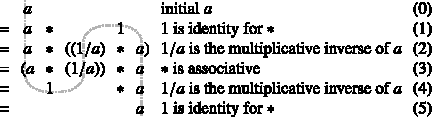
\includegraphics{diagrams/thesis/algebra-wire2.pdf}
}
\end{center}

%%%%%%%%%%%%%%%%%%%%%%%%%%%%%%%%%%%%%%%%%%%%%%%%%%%%%%%%%%%%%%%%%%%%%%%%%%%%%%
\section{Connections to Category Theory} 

We have constructed a concrete closed monoidal category. We did not use the
Int-construction which requires an existing trace operator. We inherit a lot
of constructions for free: name, coname, trace, etc.

We have constructed a good candidate for pointed homotopy category.

%%%%%%%%%%%%%%%%%%%%%%%%%%%%%%%%%%%%%%%%%%%%%%%%%%%%%%%%%%%%%%%%%%%%%%%%%%%%%%
\section{Connections to Resource Interpretation} 

We can interpret $\times$ as parallel computations (i.e., as computations
occurring simultaneously in different regions in space). So a value of type
$A \times B$ consists of two values occupying two different space locations,
e.g., two different memory locations. With that perspective, a value of type
$\frac{1}{A}$ consists of a small dictionary that stores all the values of
type $A$ and can shuffle them around.

%%%%%%%%%%%%%%%%%%%%%%%%%%%%%%%%%%%%%%%%%%%%%%%%%%%%%%%%%%%%%%%%%%%%%%%%%%%%%%
\section{Connections to Homotopy Theory} 

The connection between type theory and homotopy theory raises some
interesting questions. What do the various shapes (spheres, tori, etc.) have
to go with programming? Our answer is that they represent a class
of \emph{functions}: isomorphisms.

We have constructed a good candidate for pointed homotopy category.

%%%%%%%%%%%%%%%%%%%%%%%%%%%%%%%%%%%%%%%%%%%%%%%%%%%%%%%%%%%%%%%%%%%%%%%%%%%%%%
\section{Connections to Physics and Quantum Computing} 

The dual vector space in quantum mechanics and its role in quantum
computing. The fact that $\eta$ and $\epsilon$ are dual is essentially the
teleportation algorithm. We can give it a computational interpretation in
terms of backtracking.

One understanding of quantum computing is that it exploits the laws of physics
to build faster machines (perhaps). Another more foundational understanding
is that it provides a computational interpretation of physics, and in
particular directly addresses the question of interpretation of quantum
mechanics. In a little known document, Rozas~\cite{Rozas:1987:CMO:889539}
uses continuations to implement the transactional interpretation of quantum
mechanics~\cite{transactional} which includes as its main ingredient a
fixpoint calculation between waves or particles traveling forwards and
backwards in time. Our work sheds no light on whether this interpretation is
the ``right one'' but it is interesting that we can directly realize it using
the primitives of our language.

The multiplicative structure has a direct connection to entangled quantum
particles, or perhaps entangled particles and anti-particles.  The idea of
entanglement, that an action on one particle is ``instantaneously''
communicated to the other, is analogous to how unifying one value affects its
dual pair which is possibly in another part of the computation.  Again our
model sheds no light on whether this is related to how nature computes but it
is again interesting that we can directly realize the idea.

%%%%%%%%%%%%%%%%%%%%%%%%%%%%%%%%%%%%%%%%%%%%%%%%%%%%%%%%%%%%%%%%%%%%%%%%%%%%%%
\section{Connections to Information Theory} 

We have given classic computational interpretations to negative
information~\cite{negative-information} and negative
entropy~\cite{negative-entropy}.

%%%%%%%%%%%%%%%%%%%%%%%%%%%%%%%%%%%%%%%%%%%%%%%%%%%%%%%%%%%%%%%%%%%%%%%%%%%%%%
\section{Speculative Connections} 

Negative types, square root types, and imaginary types have also appeared in
the literature: we proceed with a simple explanation. We have so far extended
the set of types to be the positive rational numbers. Now we will push this
and extend the set of types to algebraic numbers. In other words, we will
allow datatypes defined by arbitrary polynomials and allow the roots of such
polynomials to be types.

Consider first an example in which we want to compute with the sides of a
rectangle whose area is 91 and whose length is longer than its width by 6
units. One can solve the quadratic equation to determine that the sides are 7
and 13 and proceed. This however prematurely forces us to globally solve the
constraint. Instead we can let the two sides of the rectangle be $x$ and
$x+6$ and use the following equation to capture the desired constraint:
\[
x^2 + 6x - 91 = 0
\]
The equation introduces an isomorphism between the type $x^2 + 6x - 91$ and
the type $0$. We can now proceed to compute with the unknown $x$, being
assured that in a closed program, our computation will eventually be
consistent with the solution of the algebraic equation. 

Previously the most famous example of a similar nature is the puzzling
isomorphism that one can establish between seven binary trees and one.
A binary tree is defined by the datatype
\[
x = 1 + x * x 
\]
which can be rearranged to the polynomial equation $x^2 - x + 1 = 0$. By
algebraic manipulation we can reason as follows:
\[\begin{array}{rclclclcl}
x^3 &=& x^2 x &=& (x-1) x &=& x^2 - x &=& -1 \\
x^6 &=& 1 \\
x^7 &=& x^6 x &=& x
\end{array}\]
Fiore poses the question of why such algebraic manipulation would make sense
type theoretically but states that even though some of the intermediate steps
make no sense, the final equivalence is valid and can be used to actually
construct an isomorphism between $x^7$ the type of seven binary trees 
and $x$ the type of binary trees.

Discussion of possible polynomials:
\begin{itemize}
\item $b=1+1$. Boring.
\item $b=b+1$. That introduces the natural numbers. No solution for this
  polynomial over the algebraic numbers. We must extend the numbers with
  $\omega$ to get a solution. We reject this in this paper and prefer to
  stick to algebraic numbers. The advantage is that all the isomorphisms are
  valid numerically. With the above type we could subtract $b$ from both
  sides to show that $0=1$ which is nonsense. We can however have infinite
  types as long as they have algebraic solutions.
\item $b^2=2$ or $b = \pm \sqrt{2}$. We have introduced the square root of a
  boolean! If we had superpositions, we could then write a function that
  performs the square root of negation in the sense that applying it twice
  would be equivalent to boolean negation.
\end{itemize}

\paragraph*{Geometry of Interaction (GoI).}
Geometry of Interaction was developed by Girard~\cite{girard1989geometry} as
part of the development of linear logic. It was given a computational
interpretation by Abramsky and
Jagadeesan~\cite{Abramsky:1994:NFG:184662.184664}, and was developed into a
reversible model of computing by
Mackie~\cite{Mackie2011,DBLP:conf/popl/Mackie95}. Preliminary investigations
suggest that many of the GoI machine constructions can be simulated by
treating Mackie's bi-directional wires as pairs of wires and replacing the
machine's global state with a typed value on the wire that captures the
appropriate state. This connection is exciting because when viewed through a
Curry-Howard lens it suggests that the logical interpretation of would be a
linear-like logic with a notion of resource preservation and with a natural
computational interpretation.

\paragraph*{Computing in the Field of Algebraic Numbers.}
\label{sec:algebraic-field}
Algebraically, the addition of fractional types corresponds to a move from a
ring-like structure to a full field. Our language captures the structure of
one particular field: that of the rational numbers. As we have seen,
computation in this field is quite expressive and interesting and yet, it has
two fundamental limitations. First it cannot express any recursive type, and
second it cannot express any datatype definitions. We believe these to be two
orthogonal extensions: recursive types were considered in our previous
paper~\cite{James:2012:IE:2103656.2103667}; arbitrary datatypes are however
even more exciting that plain rationals as each datatype definition can be
viewed as a polynomial (see below) which essentially means that we start
computing in the field of algebraic numbers, which includes square roots and
imaginary numbers. As crazy as it might seem, the type $\sqrt{2}$ and even
the type $(1/2)+i(\sqrt{3}/2)$ ``make sense.''  In fact the latter type is
the solution to the polynomial $x^2-x+1=0$ which if re-arranged looks like
$x=1+x*x$ and perhaps more familiarly as the datatype of binary trees $\mu
x.(1+x*x)$. These types happen to have been studied extensively following a
paper by Blass~\cite{seventrees} which used the above datatype of trees to
infer an isomorphism between seven binary trees and one!

We have confirmed that we can extend our language with the datatype
declaration for binary trees and build a witness for this isomorphism that
works as expected. However not every isomorphism constructed from algebraic
manipulation is computationally meaningful. To understand the issue in more
detail, consider the following algebraically valid proof of the isomorphism
in question:
\[\begin{array}{rclclclcl}
x^3 &=& x^2 x &=& (x-1) x &=& x^2 - x &=& -1 \\
x^6 &=& 1 \\
x^7 &=& x^6 x &=& x
\end{array}\]
The question is why such an algebraic manipulation makes sense type
theoretically, even though the intermediate step asking for an isomorphism
between $x^6$ and $1$ has no computational context. In our setting, this
isomorphism can be constructed but it diverges on all inputs (in both
ways). This suggests that, in the field of algebraic numbers, some algebraic
manipulations are somehow ``more constructive'' than others.

A related issue is that not all meaningful recursive types are meaningful
polynomials. For instance $\textsf{nat}=\mu x.(1+x)$ implies the polynomial
$x=1+x$ which has no algebraic solutions without appeal to more complex
structures with limits etc.

%%%%%%%%%%%%%%%%%%%%%%%%%%%%%%%%%%%%%%%%%%%%%%%%%%%%%%%%%%%%%%%%%%%%%%%%%%%%%%
\section{Conclusions and Future Work} 

This is cool and deep.

\paragraph*{Declarative Continuations.} 
In his Masters thesis~\cite{Filinski:1989:DCI:648332.755574}, Filinski
proposes that continuations are a \emph{declarative} concept. He,
furthermore, introduces a symmetric extension of the $\lambda$-calculus in
which call-by-value is dual to call-by-name and values are dual to
continuations. In more detail, the symmetric calculus contains a ``value''
fragment and a ``continuation'' fragment which are mirror images. Pairs and
sums are treated as duals in the sense that the ``value'' fragment includes
pairs whose mirror image in the ``continuation'' fragment are sums. In
contrast, our language includes pairs and sums in the value fragment and two
symmetries: one that maps the pairs to fractions and another that maps the
sums to subtractions.

\paragraph*{The Duality of Computation.}
The duality between call-by-name and call-by-value was further investigated
by Selinger using control
categories~\cite{Selinger:2001:CCD:966910.966911}. Curien and
Herbelin~\cite{Curien:2000} also introduce a calculus that exhibits
symmetries between values and continuations and between call-by-value and
call-by-name. The calculus includes the type $A-B$ which is the dual of
implication, i.e., a value of type $A-B$ is a context expecting a function of
type $A \rightarrow B$. Alternatively a value of type $A-B$ is also explained
as a \emph{pair} consisting of a value of type $A$ and a continuation of type
$B$. This is to be contrasted with our interpretation of a value of that type
as \emph{either} a value of $A$ or a demand for a value of type $B$. This
calculus was further analyzed and extended by
Wadler~\cite{Wadler:2003,DBLP:conf/rta/Wadler05}. The extension gives no
interpretation to the subtraction connective and like the original symmetric
calculus of Filinski, introduces a duality that relates sums to products and
vice-versa.

\paragraph*{Subtractive Logic.} 
Rauszer~\cite{springerlink:10.1007/BF02120864,rauszer,rauszer2} introduced a
logic which contains a dual to implication. Her work has been distilled in
the form of \emph{subtractive logic}~\cite{Crolard01} which has recently been
related to coroutines~\cite{Crolard01082004} and delimited
continuations~\cite{Ariola:2009:TFD:1743339.1743381}.  In more detail,
Crolard explains the type $A-B$ as the type of \emph{coroutines} with a local
environment of type $A$ and a continuation of type $B$. The description is
complicated by what is essentially the desire to enforce linearity
constraints so that coroutines cannot access the local environment of other
coroutines. 

\paragraph*{Negation in Classical Linear Logic} 
Filinski~\cite{Filinski92} uses the negative types of linear logic to model
continuations. Reddy~\cite{Reddy91} generalizes this idea by interpreting the
negative types of linear logic as \emph{acceptors}, which are like
continuations in the sense that they take an input and return no
output. Acceptors however are also similar in flavor to logic variables:
they can be created and instantiated later once their context of use is
determined. Although a formal connection is lacking, it is clear that, at an
intuitive level, acceptors are entities that combine elements of our negative
and fractional types.

\paragraph*{The Lambek-Grishin Calculus.} The ``parsing-as-deduction'' style
of linguistic analysis uses the Lambek-Grishin calculus with the following
types: product, left division, right division, sum, right difference, and
left difference~\cite{Bernardi:2010:CSL:1749618.1749689}. The division and
difference types are similar to our types but because the calculus lacks
commutativity and associativity and only has limited notions of
distributivity, each connective needs a left and right version. The
Lambek-Grishin exhibits two notions of symmetry but they are unrelated to our
notions. In particular, the first notion of symmetry expresses commutativity
and the second relates products to sums and divisions to subtractions. In
contrast, our two symmetries relate sums to subtractions and products to
divisions.

%%%%%%%%%%%%%%%%%%%%%%%%%%%%%%%%%%%%%%%%%%%%%%%%%%%%%%%%%%%%%%%%%%%%%%%%%%%%%%
\section*{Acknowledgments}

This material is based upon work supported by the National Science Foundation
under Grant No. 1217454. We would like to specially thank Roshan James and
Zachary Sparks for their contributions to early stages of this work. 

%%%%%%%%%%%%%%%%%%%%%%%%%%%%%%%%%%%%%%%%%%%%%%%%%%%%%%%%%%%%%%%%%%%%%%%%%%%%%%
\bibliographystyle{plain}
\bibliography{cites}
\end{document}

